\documentclass[notheorems, handout]{beamer}

\usetheme{warsaw}
\setbeamertemplate{page number in head/foot}[totalframenumber]
\setbeamertemplate{headline}{}
\setbeamertemplate{navigation symbols}{}
\usefonttheme[onlymath]{serif}

\usepackage[utf8]{inputenc}
\usepackage[english]{babel}

\usepackage{graphicx,subcaption,ragged2e}
\usepackage{tikz}
\usepackage{bm}

\setbeamercolor{bluetext_color}{fg=blue}
\newcommand{\bluetext}[1]{{\usebeamercolor[fg]{bluetext_color}#1}}

\usetikzlibrary{shapes.geometric, arrows}
\tikzstyle{arrow} = [thick,->,>=stealth]

\title[MC-SSA for extracting weak signals]{Monte Carlo SSA for extracting weak signals}

\author[E. Poteshkin, N. Golyandina]{Egor Poteshkin, Nina Golyandina}

\institute[Saint Petersburg State University]{%
	\small
	Saint Petersburg State University\\
	Department of Statistical Modeling}

\date{\\CDAM'2025\\September 24, 2025, Minsk, Belarus}

\subject{Talks}	

%new calligraphic font for subspaces 
\usepackage{euscript}
\newcommand{\cA}{\EuScript{A}}
\newcommand{\cB}{\EuScript{B}}
\newcommand{\cC}{\EuScript{C}}
\newcommand{\cD}{\EuScript{D}}
\newcommand{\cE}{\EuScript{E}}
\newcommand{\cF}{\EuScript{F}}
\newcommand{\cG}{\EuScript{G}}
\newcommand{\cH}{\EuScript{H}}
\newcommand{\cI}{\EuScript{I}}
\newcommand{\cJ}{\EuScript{J}}
\newcommand{\cK}{\EuScript{K}}
\newcommand{\cL}{\EuScript{L}}
\newcommand{\cM}{\EuScript{M}}
\newcommand{\cN}{\EuScript{N}}
\newcommand{\cO}{\EuScript{O}}
\newcommand{\cP}{\EuScript{P}}
\newcommand{\cQ}{\EuScript{Q}}
\newcommand{\cR}{\EuScript{R}}
\newcommand{\cS}{\EuScript{S}}
\newcommand{\cT}{\EuScript{T}}
\newcommand{\cU}{\EuScript{U}}
\newcommand{\cV}{\EuScript{V}}
\newcommand{\cW}{\EuScript{W}}
\newcommand{\cX}{\EuScript{X}}
\newcommand{\cY}{\EuScript{Y}}
\newcommand{\cZ}{\EuScript{Z}}

%font for text indices like transposition X^\mathrm{T}
\newcommand{\rmA}{\mathrm{A}}
\newcommand{\rmB}{\mathrm{B}}
\newcommand{\rmC}{\mathrm{C}}
\newcommand{\rmD}{\mathrm{D}}
\newcommand{\rmE}{\mathrm{E}}
\newcommand{\rmF}{\mathrm{F}}
\newcommand{\rmG}{\mathrm{G}}
\newcommand{\rmH}{\mathrm{H}}
\newcommand{\rmI}{\mathrm{I}}
\newcommand{\rmJ}{\mathrm{J}}
\newcommand{\rmK}{\mathrm{K}}
\newcommand{\rmL}{\mathrm{L}}
\newcommand{\rmM}{\mathrm{M}}
\newcommand{\rmN}{\mathrm{N}}
\newcommand{\rmO}{\mathrm{O}}
\newcommand{\rmP}{\mathrm{P}}
\newcommand{\rmQ}{\mathrm{Q}}
\newcommand{\rmR}{\mathrm{R}}
\newcommand{\rmS}{\mathrm{S}}
\newcommand{\rmT}{\mathrm{T}}
\newcommand{\rmU}{\mathrm{U}}
\newcommand{\rmV}{\mathrm{V}}
\newcommand{\rmW}{\mathrm{W}}
\newcommand{\rmX}{\mathrm{X}}
\newcommand{\rmY}{\mathrm{Y}}
\newcommand{\rmZ}{\mathrm{Z}}

%tt font for time series
\newcommand{\tA}{\mathsf{A}}
\newcommand{\tB}{\mathsf{B}}
\newcommand{\tC}{\mathsf{C}}
\newcommand{\tD}{\mathsf{D}}
\newcommand{\tE}{\mathsf{E}}
\newcommand{\tF}{\mathsf{F}}
\newcommand{\tG}{\mathsf{G}}
\newcommand{\tH}{\mathsf{H}}
\newcommand{\tI}{\mathsf{I}}
\newcommand{\tJ}{\mathsf{J}}
\newcommand{\tK}{\mathsf{K}}
\newcommand{\tL}{\mathsf{L}}
\newcommand{\tM}{\mathsf{M}}
\newcommand{\tN}{\mathsf{N}}
\newcommand{\tO}{\mathsf{O}}
\newcommand{\tP}{\mathsf{P}}
\newcommand{\tQ}{\mathsf{Q}}
\newcommand{\tR}{\mathsf{R}}
\newcommand{\tS}{\mathsf{S}}
\newcommand{\tT}{\mathsf{T}}
\newcommand{\tU}{\mathsf{U}}
\newcommand{\tV}{\mathsf{V}}
\newcommand{\tW}{\mathsf{W}}
\newcommand{\tX}{\mathsf{X}}
\newcommand{\tY}{\mathsf{Y}}
\newcommand{\tZ}{\mathsf{Z}}

%bf font for matrices
\newcommand{\bfA}{\mathbf{A}}
\newcommand{\bfB}{\mathbf{B}}
\newcommand{\bfC}{\mathbf{C}}
\newcommand{\bfD}{\mathbf{D}}
\newcommand{\bfE}{\mathbf{E}}
\newcommand{\bfF}{\mathbf{F}}
\newcommand{\bfG}{\mathbf{G}}
\newcommand{\bfH}{\mathbf{H}}
\newcommand{\bfI}{\mathbf{I}}
\newcommand{\bfJ}{\mathbf{J}}
\newcommand{\bfK}{\mathbf{K}}
\newcommand{\bfL}{\mathbf{L}}
\newcommand{\bfM}{\mathbf{M}}
\newcommand{\bfN}{\mathbf{N}}
\newcommand{\bfO}{\mathbf{O}}
\newcommand{\bfP}{\mathbf{P}}
\newcommand{\bfQ}{\mathbf{Q}}
\newcommand{\bfR}{\mathbf{R}}
\newcommand{\bfS}{\mathbf{S}}
\newcommand{\bfT}{\mathbf{T}}
\newcommand{\bfU}{\mathbf{U}}
\newcommand{\bfV}{\mathbf{V}}
\newcommand{\bfW}{\mathbf{W}}
\newcommand{\bfX}{\mathbf{X}}
\newcommand{\bfY}{\mathbf{Y}}
\newcommand{\bfZ}{\mathbf{Z}}

%bb font for standard spaces and expectation
\newcommand{\bbA}{\mathbb{A}}
\newcommand{\bbB}{\mathbb{B}}
\newcommand{\bbC}{\mathbb{C}}
\newcommand{\bbD}{\mathbb{D}}
\newcommand{\bbE}{\mathbb{E}}
\newcommand{\bbF}{\mathbb{F}}
\newcommand{\bbG}{\mathbb{G}}
\newcommand{\bbH}{\mathbb{H}}
\newcommand{\bbI}{\mathbb{I}}
\newcommand{\bbJ}{\mathbb{J}}
\newcommand{\bbK}{\mathbb{K}}
\newcommand{\bbL}{\mathbb{L}}
\newcommand{\bbM}{\mathbb{M}}
\newcommand{\bbN}{\mathbb{N}}
\newcommand{\bbO}{\mathbb{O}}
\newcommand{\bbP}{\mathbb{P}}
\newcommand{\bbQ}{\mathbb{Q}}
\newcommand{\bbR}{\mathbb{R}}
\newcommand{\bbS}{\mathbb{S}}
\newcommand{\bbT}{\mathbb{T}}
\newcommand{\bbU}{\mathbb{U}}
\newcommand{\bbV}{\mathbb{V}}
\newcommand{\bbW}{\mathbb{W}}
\newcommand{\bbX}{\mathbb{X}}
\newcommand{\bbY}{\mathbb{Y}}
\newcommand{\bbZ}{\mathbb{Z}}

%got font for any case
\newcommand{\gA}{\mathfrak{A}}
\newcommand{\gB}{\mathfrak{B}}
\newcommand{\gC}{\mathfrak{C}}
\newcommand{\gD}{\mathfrak{D}}
\newcommand{\gE}{\mathfrak{E}}
\newcommand{\gF}{\mathfrak{F}}
\newcommand{\gG}{\mathfrak{G}}
\newcommand{\gH}{\mathfrak{H}}
\newcommand{\gI}{\mathfrak{I}}
\newcommand{\gJ}{\mathfrak{J}}
\newcommand{\gK}{\mathfrak{K}}
\newcommand{\gL}{\mathfrak{L}}
\newcommand{\gM}{\mathfrak{M}}
\newcommand{\gN}{\mathfrak{N}}
\newcommand{\gO}{\mathfrak{O}}
\newcommand{\gP}{\mathfrak{P}}
\newcommand{\gQ}{\mathfrak{Q}}
\newcommand{\gR}{\mathfrak{R}}
\newcommand{\gS}{\mathfrak{S}}
\newcommand{\gT}{\mathfrak{T}}
\newcommand{\gU}{\mathfrak{U}}
\newcommand{\gV}{\mathfrak{V}}
\newcommand{\gW}{\mathfrak{W}}
\newcommand{\gX}{\mathfrak{X}}
\newcommand{\gY}{\mathfrak{Y}}
\newcommand{\gZ}{\mathfrak{Z}}

%old calligraphic font
\newcommand{\calA}{\mathcal{A}}
\newcommand{\calB}{\mathcal{B}}
\newcommand{\calC}{\mathcal{C}}
\newcommand{\calD}{\mathcal{D}}
\newcommand{\calE}{\mathcal{E}}
\newcommand{\calF}{\mathcal{F}}
\newcommand{\calG}{\mathcal{G}}
\newcommand{\calH}{\mathcal{H}}
\newcommand{\calI}{\mathcal{I}}
\newcommand{\calJ}{\mathcal{J}}
\newcommand{\calK}{\mathcal{K}}
\newcommand{\calL}{\mathcal{L}}
\newcommand{\calM}{\mathcal{M}}
\newcommand{\calN}{\mathcal{N}}
\newcommand{\calO}{\mathcal{O}}
\newcommand{\calP}{\mathcal{P}}
\newcommand{\calQ}{\mathcal{Q}}
\newcommand{\calR}{\mathcal{R}}
\newcommand{\calS}{\mathcal{S}}
\newcommand{\calT}{\mathcal{T}}
\newcommand{\calU}{\mathcal{U}}
\newcommand{\calV}{\mathcal{V}}
\newcommand{\calW}{\mathcal{W}}
\newcommand{\calX}{\mathcal{X}}
\newcommand{\calY}{\mathcal{Y}}
\newcommand{\calZ}{\mathcal{Z}}


\begin{document}
\begin{frame}[plain]
	\titlepage
	\note{Научный руководитель  д.ф.-м.н., профессор Голяндина\,Н.\,Э.,\\
		кафедра статистического моделирования}
\end{frame}

\begin{frame}{Is There a Signal?}
	\begin{figure}
		\centering
		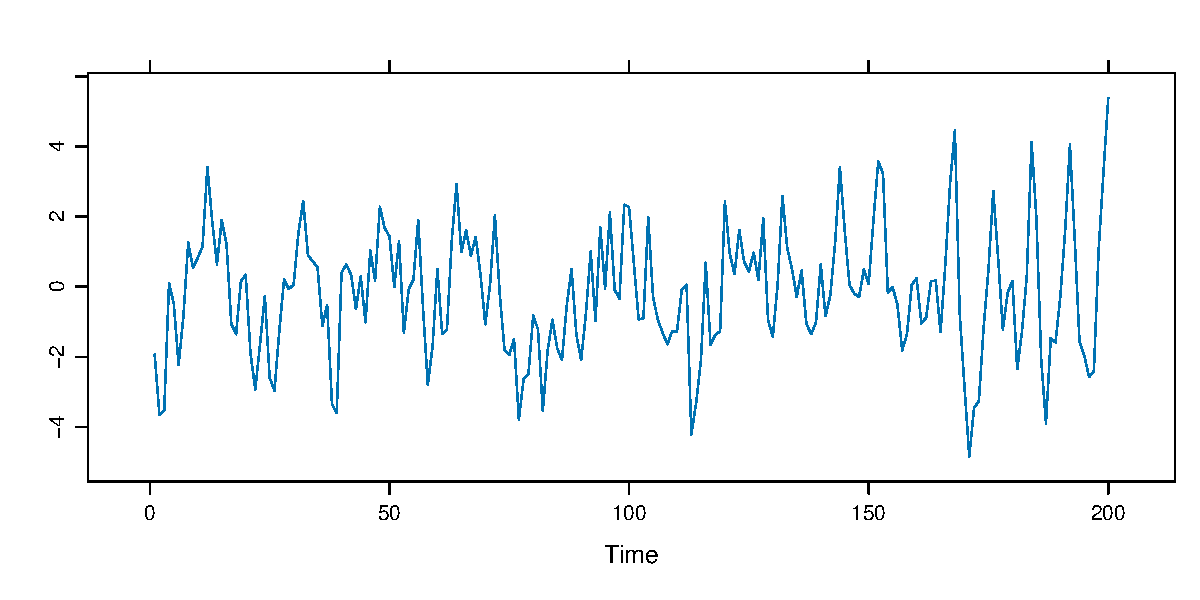
\includegraphics[width=\textwidth]{img/noise_ts.pdf}
	\end{figure}
	\bluetext{Question}: is it pure noise, or is there a signal?
\end{frame}

\begin{frame}{Problem Statement}
	Let $\tX=(x_1,\ldots,x_N)$, $x_i\in \mathbb{R}$ be a time series.\medskip

	\bluetext{Given}: $\tX=\tT + \tH + \tR$, where $\tT$ is a trend, $\tH$ is a periodic component, and $\tR$ is a noise.\medskip

	\bluetext{Problems}:
	\begin{enumerate}
		\item How to test for the presence of a signal $\tS=\tT + \tH$?
		\item How to extract the signal $\tS$, if present?\medskip
	\end{enumerate}

	\bluetext{Methods}:
	\begin{enumerate}
		\item Monte Carlo SSA (MC-SSA)~[Allen and Smith, 1996]~--- tests $H_0:\tS=0$.
		\item Singular spectrum analysis\linebreak(SSA)~[Golyandina, Nekrutkin and Zhigljavsky, 2001].\medskip
	\end{enumerate}
	\bluetext{Goal}: to implement an algorithm for automatic signal extraction based on MC-SSA
\end{frame}

\begin{frame}{Notations \& Known Results: Embedding and Hankelization}
	For $\tX=(x_1,\ldots,x_N)$, fix $L$ ($1<L<N$).\medskip

	\emph{Embedding operator} $\cT_\text{SSA}$:
	\begin{equation*}
		\cT_{\text{SSA}}(\tX)=\bfX=\begin{pmatrix}
			x_1    & x_2     & \cdots & x_K     \\
			x_2    & x_3     & \cdots & x_{K+1} \\
			\vdots & \vdots  & \ddots & \vdots  \\
			x_L    & x_{L+1} & \cdots & x_N
		\end{pmatrix},
	\end{equation*}
	where $K=N-L+1$.\medskip

	\emph{Hankelization operator} $\cH$~--- averaging the matrix over its anti-diagonals.
\end{frame}

\begin{frame}{Notations \& Known Results: The SSA Algorithm}
	\bluetext{Input}: time series $\tX=(x_1,\ldots,x_N)$.\\

	\bluetext{Parameters}: window length $L$, index set $I\subset\{1,\ldots,d\}$. \\

	\bluetext{Output}: signal estimate.\medskip

	\begin{figure}
		\scalebox{0.5}{
			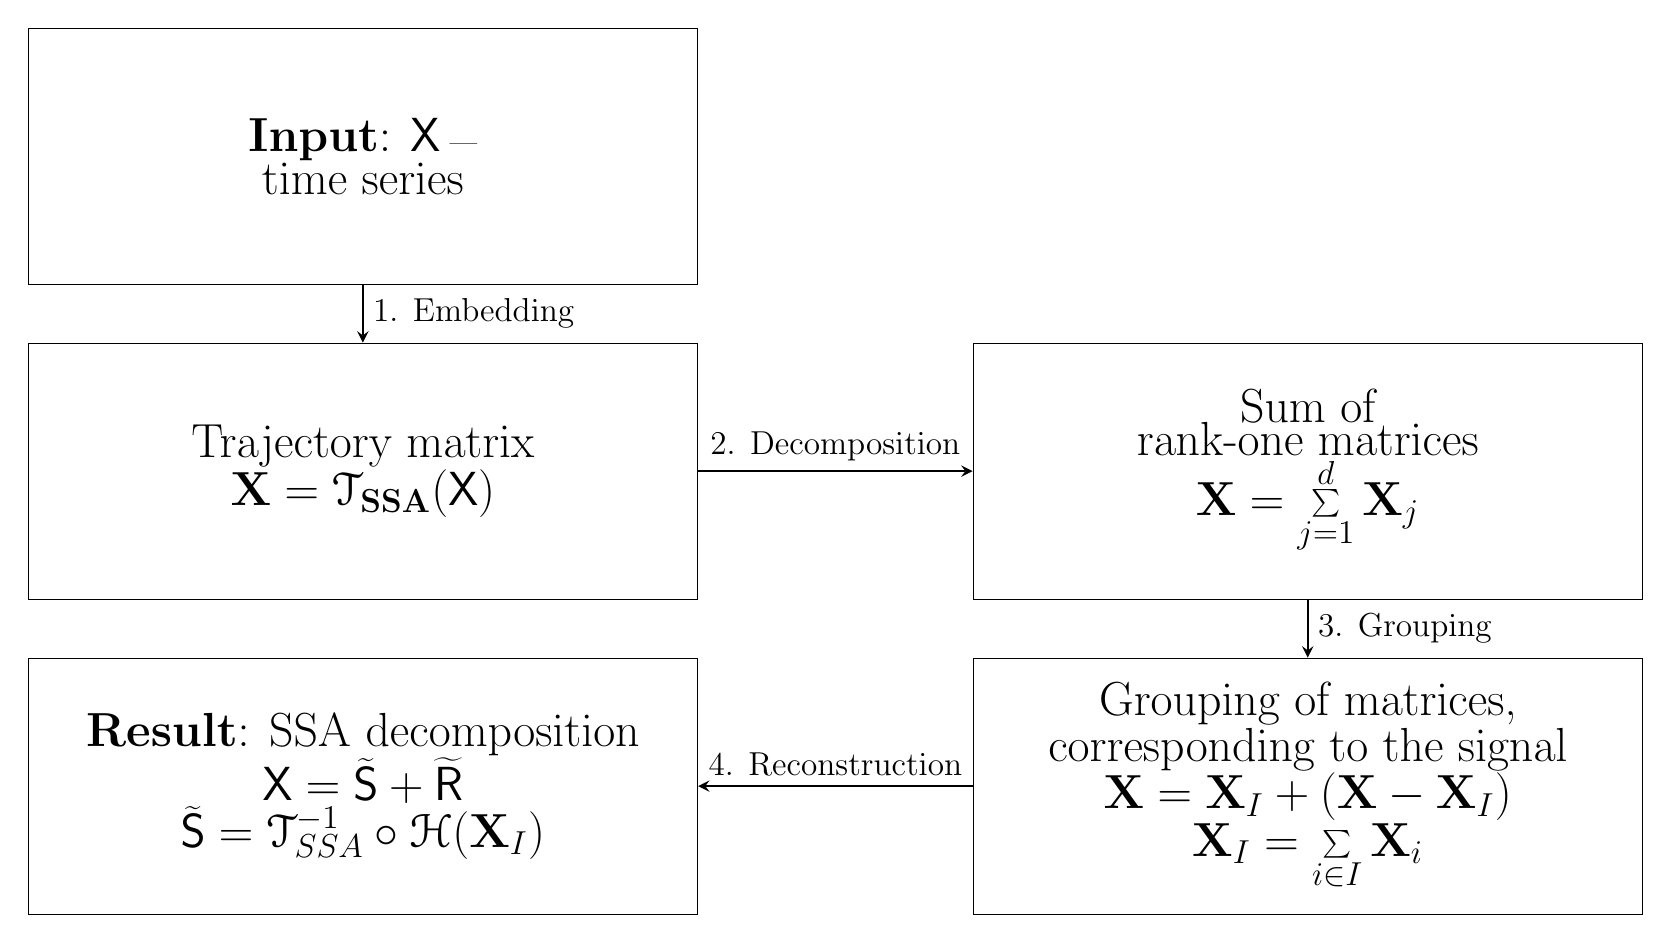
\begin{tikzpicture}[node distance=2cm]
				\node[draw, align=center, minimum width=8.5cm, minimum height=3.25cm](1){{\LARGE\textbf{Input}: $\tX$}~---\\\LARGE time series};
				\node[draw, align=center, minimum width=8.5cm, minimum height=3.25cm, below of=1, yshift=-2cm](2){{\LARGE Trajectory matrix}\\ \LARGE $\bf{X}=\cT_{\text{SSA}}(\tX)$};
				\node[draw, align=center, minimum width=8.5cm, minimum height=3.25cm, right of=2, xshift=10cm](3){\LARGE Sum of\\ \LARGE rank-one matrices\\ \LARGE$\bfX=\sum\limits_{j=1}^d\bfX_j$};
				\node[draw, align=center, minimum width=8.5cm, minimum height=3.25cm, below of=3, yshift=-2cm](4){\LARGE Grouping of matrices,\\ \LARGE corresponding to the signal\\ \LARGE$\bfX=\bfX_{I}+(\bfX-\bfX_{I})$\\\LARGE$\bfX_{I}=\sum\limits_{i\in I}\bfX_i$};
				\node[draw, align=center, minimum width=8.5cm, minimum height=3.25cm, below of=2, yshift=-2cm](5){\LARGE\textbf{Result}: SSA decomposition\\\LARGE$\tX=\widetilde\tS+\widetilde{\tR}$\\\LARGE$\widetilde\tS=\cT_\text{SSA}^{-1}\circ\cH(\bfX_{I})$};

				\draw[arrow](1)--node[anchor=west]{\large1. Embedding}(2);
				\draw[arrow](2)--node[anchor=south]{\large2. Decomposition}(3);
				\draw[arrow](3)--node[anchor=west]{\large3. Grouping}(4);
				\draw[arrow](4)--node[anchor=south]{\large4. Reconstruction}(5);
			\end{tikzpicture}}
	\end{figure}
\end{frame}

\begin{frame}{Example: Applying SSA}
	\begin{figure}
		\centering
		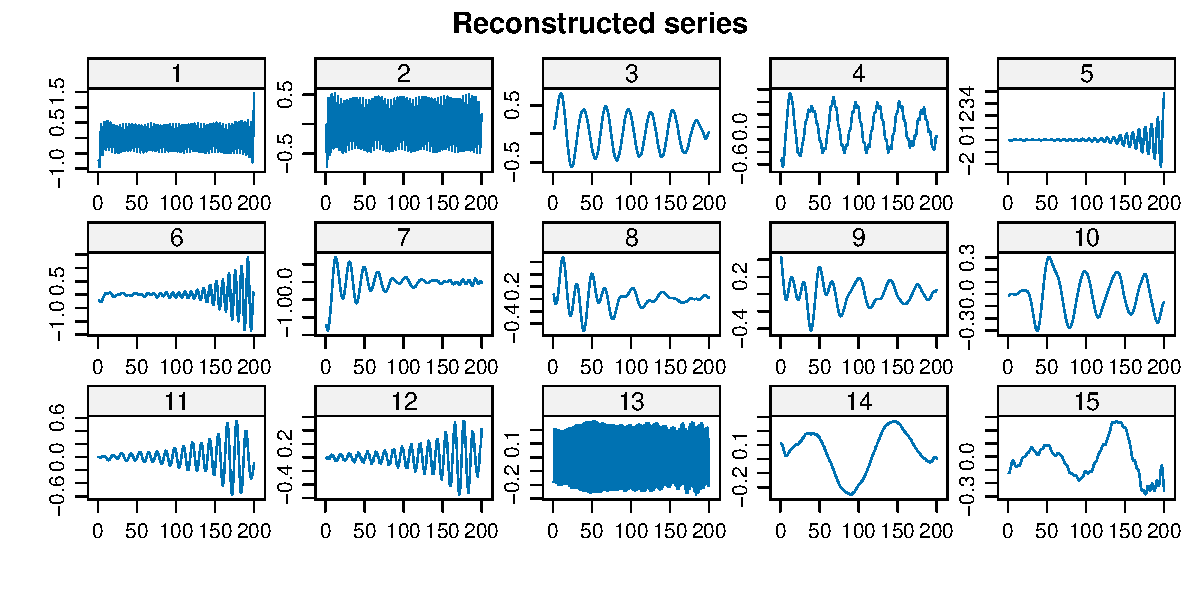
\includegraphics[width=\textwidth]{../paper/img/reconstructed_ts.pdf}
		\caption{Elementary reconstructed components ($L=100$)}
	\end{figure}
	Components corresponding to the signal: $1$, $2$, $5$, $6$ and $13$.
\end{frame}

\begin{frame}{Notations \& Known Results: Monte Carlo SSA}
	\bluetext{Input}: $\tX=\tS+\tR$, where $\tS$ is the signal and $\tR$ is a realization of a zero-mean stationary process $\bm\xi$ with spectral density $f_{\bm\theta}$.\medskip

	\bluetext{Parameters}: window length $L$, normalized vectors corresponding to specific frequencies $W_1,\ldots, W_M\in \mathbb R^L$.\medskip

	\bluetext{Test statistics}:
	$$
		\widehat p_k = \left\|\bfX^\rmT W_k\right\|^2.
	$$

	Its distribution under $H_0$ is generally unknown and is estimated via Monte Carlo.\medskip

	Multiple MC-SSA~[Golyandina, 2023]: modification with multiple comparisons correction.\medskip

	We chose sine waves with equidistant frequencies $\omega_k=k/(2L)$, $k=1,\ldots, L$ as projection vectors.
\end{frame}

\begin{frame}{Notations \& Known Results: Noise Parameters Estimation}
	Noise parameters $\bm\theta$ are generally unknown and must be estimated.\medskip

	Parameter estimates can be obtained by maximizing the Whittle's likelihood~[Whittle, 1953]:
	$$
		\ell_W(\bm\theta)=-\frac{1}{m}\sum_{j=1}^m\left(\ln f_{\bm\theta}(\omega_j)+\frac{I_N(\omega_j)}{f_{\bm\theta}(\omega_j)}\right),
	$$
	where $m=\lfloor (N-1)/2\rfloor$, $f_{\bm\theta}$ is the spectral density of $\bm\xi$, $I_N$ is the periodogram of the original series, and $\omega_j=j/N$.\medskip

	Estimation can be done on part of the spectrum: let $J=\{j_1, \ldots, j_p\}$ be frequency indices we want to exclude when estimating parameters. Then $\ell_W(\bm\theta)$ is computed only over indices $j\not\in J$.
\end{frame}

\begin{frame}{Example: Applying Monte Carlo SSA}
	$\tX=\tS+\boldsymbol{\xi}$, where $\boldsymbol{\xi}$ is red noise with parameters $\phi=0.7$ and $\sigma^2=1$, $N=200$,
	$$
		s_n=0.075\,e^{0.02n}\cos(2\pi n / 8) + 2\cos(2\pi n / 4) + 0.2\cdot (-1)^n.
	$$
	\begin{figure}
		\centering
		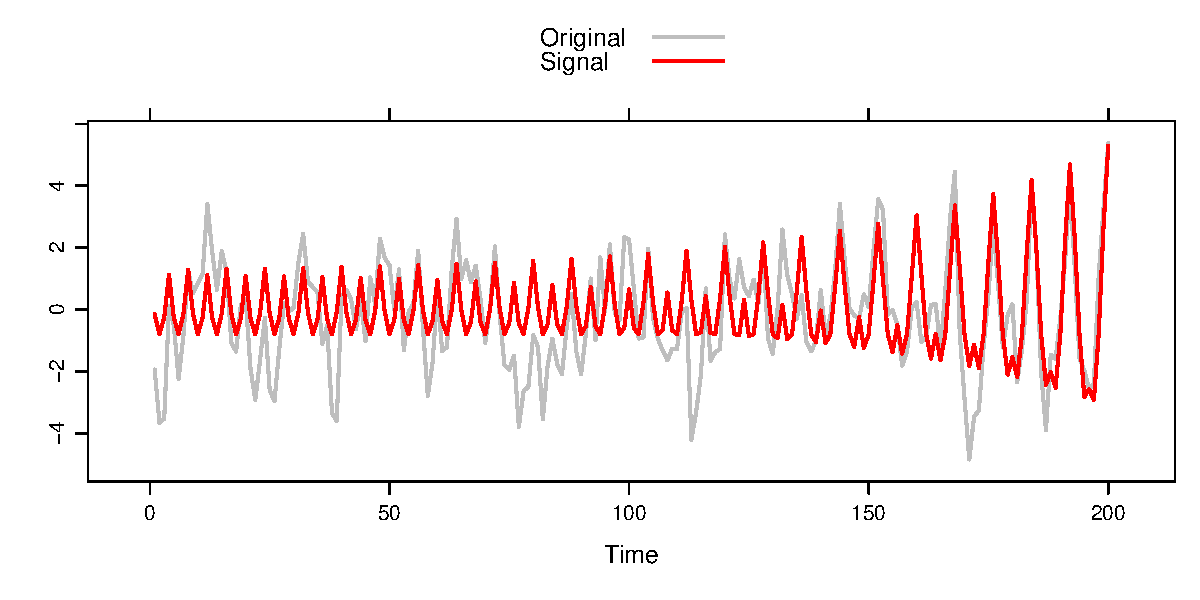
\includegraphics[width=\textwidth]{img/noise_ts_signal.pdf}
	\end{figure}
\end{frame}

\begin{frame}{Example: Applying Monte Carlo SSA}
	\begin{figure}
		\centering
		\minipage{0.5\textwidth}
		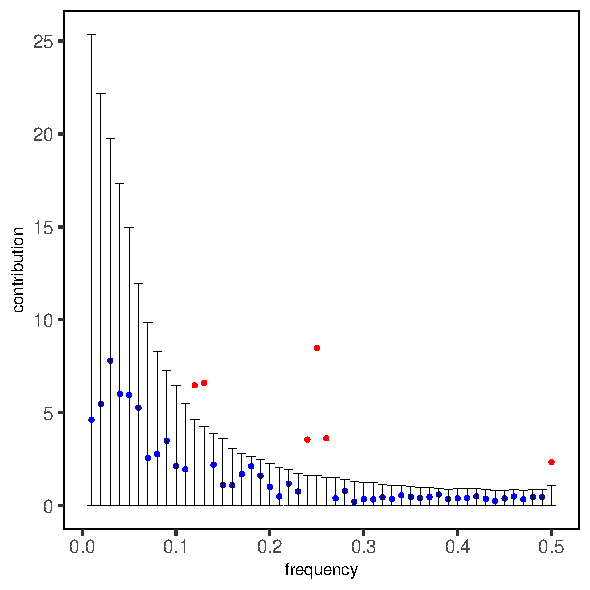
\includegraphics[width=0.9\textwidth]{img/mcssa_real.pdf}
		\caption{True noise model}
		\endminipage\hfill
		\minipage{0.5\textwidth}
		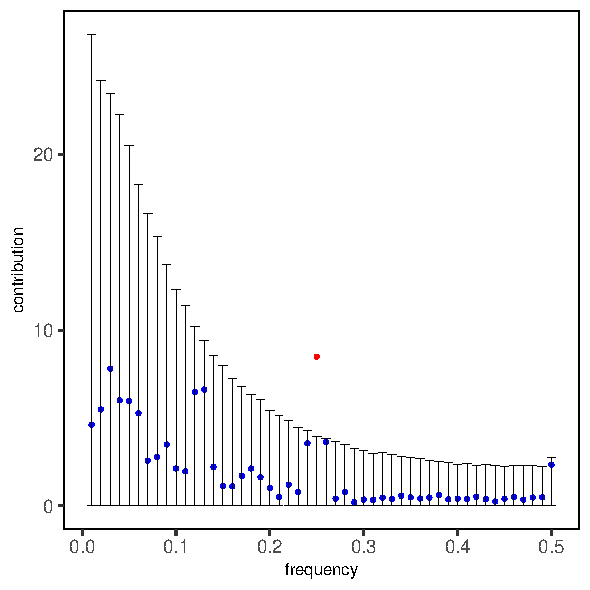
\includegraphics[width=0.9\textwidth]{img/mcssa_estimated.pdf}
		\caption{Estimated noise model}
		\endminipage
	\end{figure}
	\textcolor{red}{Problem}: not all frequencies are detected during parameter estimation.

	\bluetext{Solution}: apply the test iteratively, extracting one harmonic at a time until $H_0:\tS=0$ is no longer rejected.
\end{frame}

\begin{frame}{Notations \& Known Results: Automatic Grouping in SSA}
	For a series $\tX$ of length $N$ and $0\leqslant\omega_1\leqslant\omega_2\leqslant0.5$, define
	$$
		T(\tX; \omega_1,\omega_2)=\frac{1}{\|\tX\|^2}\sum_{k:\omega_1\leqslant k / N \leqslant \omega_2}I_N(k / N),
	$$
	where $I_N$ is the periodogram of $\tX$. \medskip

	$T(\tX; \omega_1, \omega_2)$ may be interpreted as the fraction of total contribution of frequencies within $[\omega_1, \omega_2]$.\bigskip

	Let $\omega^\star$ be a significant frequency. Then we take $[\omega_1, \omega_2]=[\omega^\star-\delta, \omega^\star + \delta]$.
\end{frame}

\begin{frame}{The autoMCSSA Algorithm}
	\begin{figure}
		\centering
		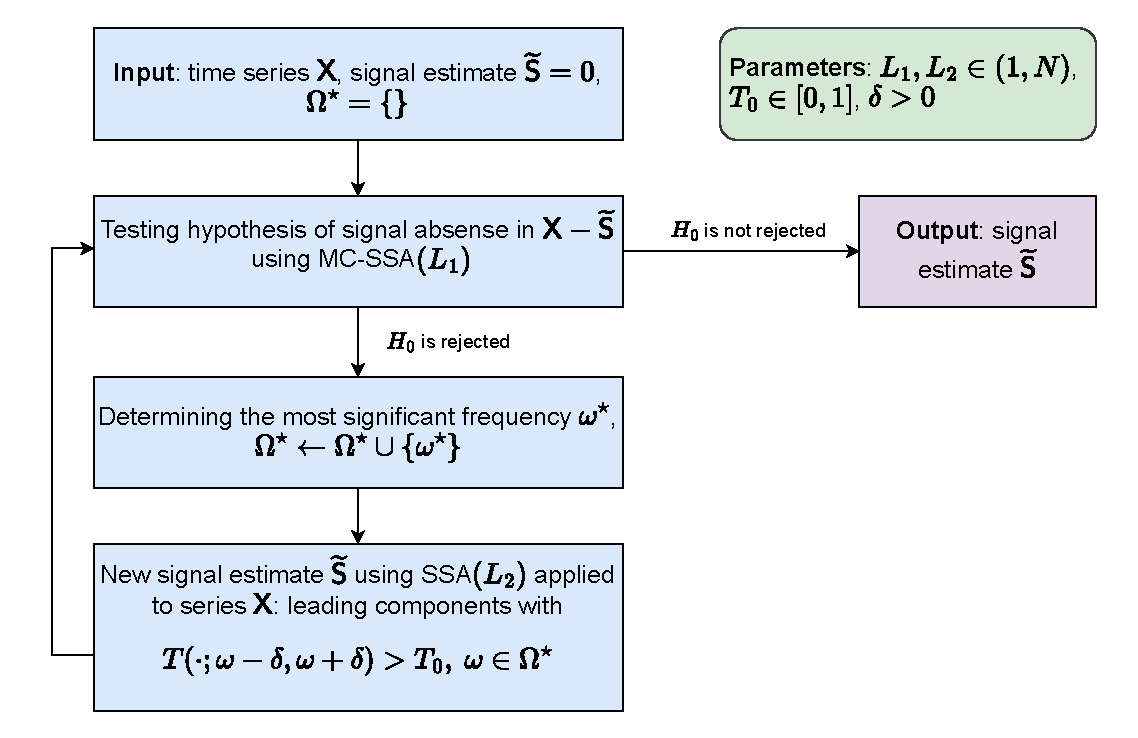
\includegraphics[width=\textwidth]{../paper/img/auto_mcssa_alg.pdf}
	\end{figure}
\end{frame}

\begin{frame}{Example: Applying autoMCSSA}
	$\tX=\tS+\boldsymbol{\xi}$, where $\boldsymbol{\xi}$ is red noise with $\phi=0.7$ and $\sigma^2=1$, $N=200$,
	$$
		s_n=0.075\,e^{0.02n}\cos(2\pi n / 8) + 2\cos(2\pi n / 4) + 0.2\cdot (-1)^n.
	$$\vspace{-2.5em}
	\begin{figure}
		\centering
		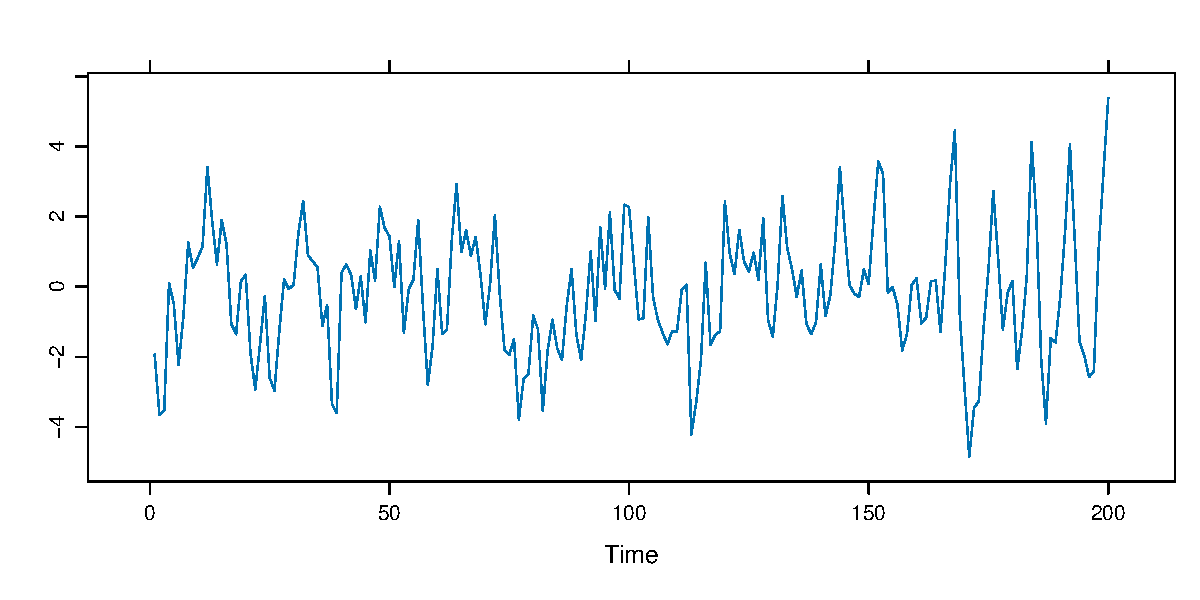
\includegraphics[width=\textwidth]{img/noise_ts.pdf}
	\end{figure}
\end{frame}

\begin{frame}{Example: Applying autoMCSSA}
	\begin{figure}
		\centering
		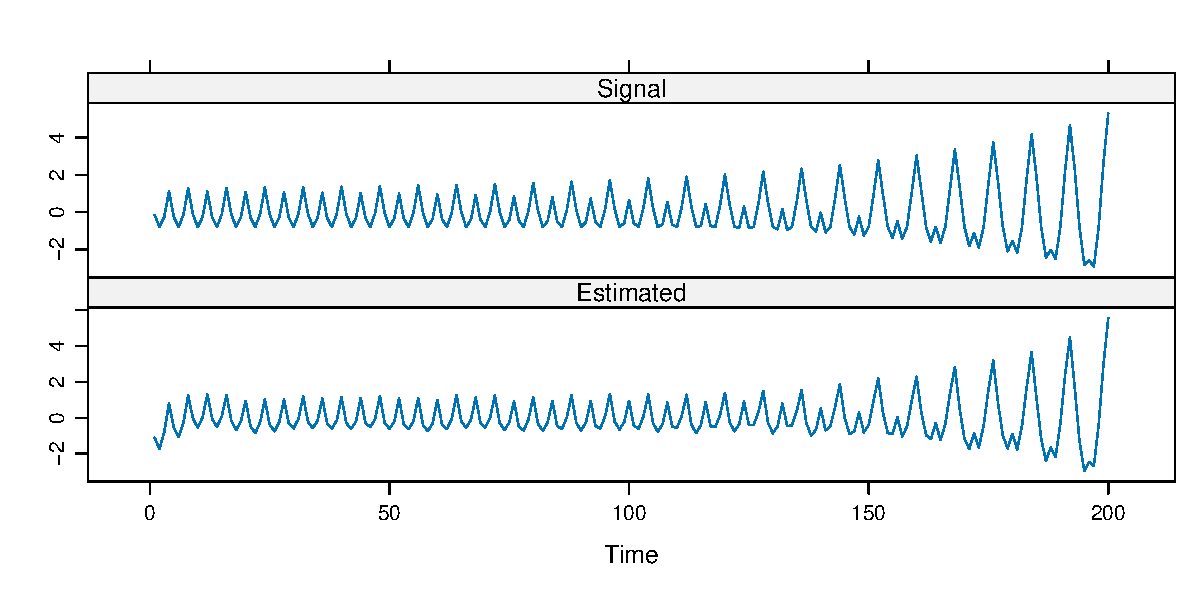
\includegraphics[width=\textwidth]{../paper/img/auto_mcssa_result.pdf}
	\end{figure}
	\textbf{Parameters}: $L_1=50$, $L_2=100$, $\delta=1/80$, $T_0=0.5$.\medskip

	\textbf{Result}: autoMCSSA correctly identified significant components ($1$, $2$, $5$, $6$ and $13$).
\end{frame}

% \begin{frame}{Численное сравнение с autoSSA}
% 	Сравним метод autoMCSSA с методом autoSSA~[Дудник, 2025].\medskip

% 	Рассмотрим временной ряд $\tX = \tS + \bm\xi$ длины $N=100$, где
% 	$$
% 	s_n=0.2e^{0.05 n}\cos(2\pi n/4) + 2\cos(2\pi n / 3) + (-1)^n,
% 	$$
% 	$\bm\xi$~--- красный шум с параметрами $\phi\in\{0, 0.5\}$, $\sigma^2=1$. Для autoMCSSA были выбраны следующие параметры:\smallskip
% 	\begin{itemize}
% 		\item Длины окна $L_1=20$ и $L_2=50$;\smallskip
% 		\item Радиус промежутка для вычисления меры $T$ $\delta = 1 / 80$;\smallskip
% 		\item Порог для меры $T$ $T_0=0.5$;\smallskip
% 		\item Максимальное количество итераций: $10$.
% 	\end{itemize}
% \end{frame}

% \begin{frame}{Численное сравнение с autoSSA}
% 	\begin{table}[h]
% 		\centering
% 		\caption{MSE выделения сигнала ($\phi=0$)}
% 		\begin{tabular}{|r|r|r|}
% 			\hline
% 			& Mean MSE & Median MSE \\ 
% 			\hline
% 			autoMCSSA & 0.15196 & 0.13921 \\ 
% 			\hline
% 			autoSSA & 0.14872 & 0.14003 \\ 
% 			\hline
% 		\end{tabular}
% 	\end{table}
% 	\begin{table}[h]
% 		\centering
% 		\caption{MSE выделения сигнала ($\phi=0.5$)}
% 		\begin{tabular}{|r|r|r|}
% 			\hline
% 			& Mean MSE & Median MSE \\ 
% 			\hline
% 			autoMCSSA & 0.11563 & 0.09038 \\ 
% 			\hline
% 			autoSSA & 0.09341 & 0.08795 \\ 
% 			\hline
% 		\end{tabular}
% 	\end{table}
% \end{frame}

\begin{frame}{Conclusions}
	To sum up, we:
	\begin{enumerate}
		\item Implemented autoMCSSA, which automatically extracts a significant signal, plus a modification of the Whittle approach using part of the spectrum.\medskip
		\item Found that autoMCSSA can extract signals whose SSA components are not necessarily dominant.\medskip
	\end{enumerate}
	In the future, we plan to formulate a strategy for selecting autoMCSSA parameters.
\end{frame}

\end{document}